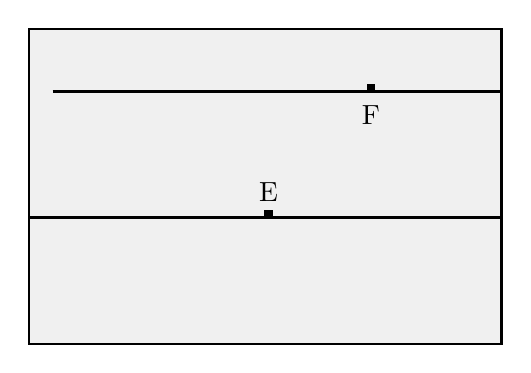
\begin{tikzpicture}[line width=0.8pt]
  % map rectangle
  \fill[gray!12] (0,0) rectangle (6,4);
  \draw (0,0) rectangle (6,4);
  % two horizontal survey lines
  \draw[line width=1pt] (0.3,3.2) -- (6,3.2);
  \draw[line width=1pt] (0,1.6) -- (6,1.6);
  % point F on upper line
  \draw[fill=black] (4.3,3.2) rectangle ++(0.08,0.08);
  \node[below] at (4.34,3.15) {F};
  % point E on lower line
  \draw[fill=black] (3.0,1.6) rectangle ++(0.08,0.08);
  \node[above] at (3.04,1.68) {E};
\end{tikzpicture}
